\documentclass[crop,tikz]{standalone}
\usepackage{amstext}
\usepackage{amssymb}
\usetikzlibrary{positioning}
\usetikzlibrary{shapes.misc}

\begin{document}


    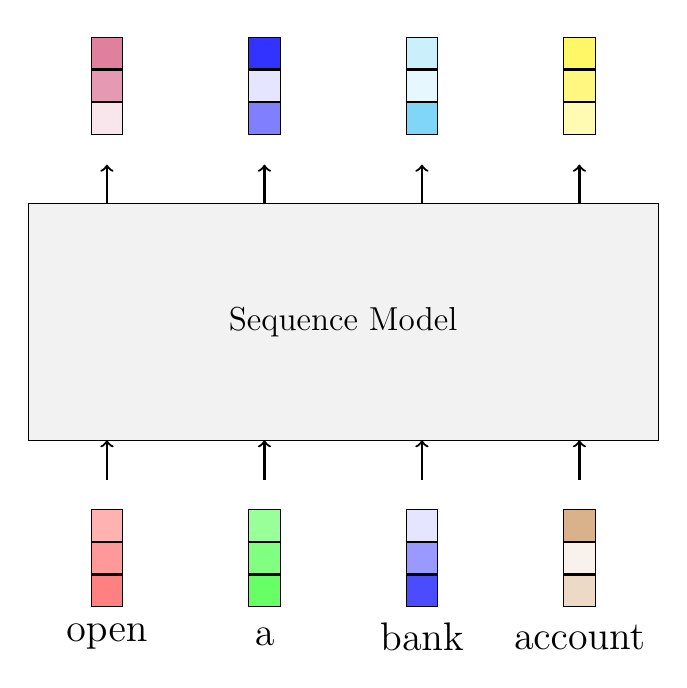
\begin{tikzpicture}[
        word/.style={font=\Large},
        embedding box/.style={draw, minimum size=0.4cm},
        stack/.style={column sep=0cm, row sep=0cm},
        model box/.style={draw, rectangle, minimum width=8cm, minimum height=3cm, fill=gray!10},
    ]

    % Define the embedding visualization with parameters
    \tikzset{
        pics/embedding/.style n args={4}{
            code={
                \matrix [stack] {
                    \node[embedding box, fill=#4!#1] {}; \\
                    \node[embedding box, fill=#4!#2] {}; \\
                    \node[embedding box, fill=#4!#3] {}; \\
                };
            }
        }
    }

    % Input words
    \node[word] (open) at (0,0) {open};
    \node[word] (a) at (2,0) {a};
    \node[word] (bank) at (4,0) {bank};
    \node[word] (account) at (6,0) {account};

    % Input embeddings with different shades
        \path (0,1) pic {embedding={30}{40}{50}{red}};  % open
        \path (2,1) pic {embedding={40}{50}{60}{green}};  % a
        \path (4,1) pic {embedding={10}{40}{70}{blue}};  % bank
        \path (6,1) pic {embedding={60}{10}{30}{brown}};  % account

    % Model box
    \node[model box] (model) at (3,4) {\large Sequence Model};

    % Output embeddings with different shades (showing contextualization)
        \path (0,7) pic {embedding={50}{40}{10}{purple}};  % contextualized open
        \path (2,7) pic {embedding={80}{10}{50}{blue}};  % contextualized a
        \path (4,7) pic {embedding={20}{10}{50}{cyan}};  % contextualized bank
        \path (6,7) pic {embedding={60}{50}{30}{yellow}};  % contextualized account

    % Draw arrows from input embeddings to model
    \draw[->, thick] (0,2) -- (0,2.5);
    \draw[->, thick] (2,2) -- (2,2.5);
    \draw[->, thick] (4,2) -- (4,2.5);
    \draw[->, thick] (6,2) -- (6,2.5);

    % Draw arrows from model to output embeddings
    \draw[->, thick] (0,5.5) -- (0,6);
    \draw[->, thick] (2,5.5) -- (2,6);
    \draw[->, thick] (4,5.5) -- (4,6);
    \draw[->, thick] (6,5.5) -- (6,6);

    \end{tikzpicture}

\end{document}
